\documentclass[aspectratio=169, 10pt]{beamer}

% Formal IEEE-style presentation theme with beautiful rounded shadows
\usetheme{Boadilla}
\usecolortheme{seahorse}
\usefonttheme{professionalfonts}

\usepackage{graphicx}
\usepackage{booktabs}
\usepackage{multirow}
\usepackage{tikz} 
\usepackage{pifont} % Added for checkmarks and crosses
\usepackage{amsmath}


% Enhancing visual appeal of lists and blocks
\setbeamertemplate{navigation symbols}{}
\setbeamertemplate{itemize item}{\color{blue!70!black}$\blacktriangleright$} 
\setbeamertemplate{itemize subitem}{\color{teal}$\bullet$}
\setbeamertemplate{caption}[numbered]
\setbeamertemplate{bibliography item}[text]
\setbeamertemplate{blocks}[rounded][shadow=true] 

% ==========================================
% HEADER LOGO CONFIGURATION
% ==========================================
\addtobeamertemplate{frametitle}{}{%
\begin{tikzpicture}[remember picture,overlay]
\node[anchor=north east, yshift=-0.1cm, xshift=-0.2cm] at (current page.north east) {%
    \IfFileExists{faculty_of_engineering.jpeg}{
\includegraphics[height=1.5cm]{faculty_of_engineering.jpeg}}{}%
};
\end{tikzpicture}}

% ==========================================
% BULLETPROOF CUSTOM FOOTER
% ==========================================
\makeatletter
\setbeamertemplate{footline}{
  \leavevmode%
  \hbox{%
  \begin{beamercolorbox}[wd=.33\paperwidth,ht=2.5ex,dp=1.125ex,center]{author in head/foot}%
    \usebeamerfont{author in head/foot}\textbf{\insertshortauthor}
  \end{beamercolorbox}%
  \begin{beamercolorbox}[wd=.38\paperwidth,ht=2.5ex,dp=1.125ex,center]{title in head/foot}%
    \usebeamerfont{title in head/foot}\textbf{Reference-Guided Few-Shot Segmentation with Foundation Models, 2026}
  \end{beamercolorbox}%
  \begin{beamercolorbox}[wd=.29\paperwidth,ht=2.5ex,dp=1.125ex,right]{date in head/foot}%
    \usebeamerfont{date in head/foot}\textbf{Page \insertframenumber{} of \inserttotalframenumber}\hspace*{2ex}
  \end{beamercolorbox}}%
  \vskip0pt%
}
\makeatother

\title[Few-Shot Image Segmentation]{Reference-Guided Few-Shot Segmentation with Foundation Models}
\subtitle{PhD Research Proposal}
\author[Omar Ahmed Fouad Hassan Wasfy]{Omar Ahmed Fouad Hassan Wasfy}
\institute[Alexandria University]{
Computer and Systems Engineering Department, Faculty of Engineering\\
 Alexandria University \\
 \vspace{1cm}
 \textbf{Supervisors: Prof. Dr. Mohamed Ismail and Prof. Dr. Nagia Ghanem}
 \\
 \vspace{0.5cm}
 \textbf{2026}
}
\date{} 

\begin{document}

% Slide 1
\begin{frame}
    \titlepage
\end{frame}

% Slide 2
\begin{frame}{Outline}
 \tableofcontents[hideallsubsections]
\end{frame}


% ==========================================
% SECTION 1: INTRODUCTION & BACKGROUND
% ==========================================
\section{Introduction \& Background}

% Slide 3
\begin{frame}{Top-Tier Venues Referenced in This Presentation}
\begin{columns}[T]
    \begin{column}{0.48\textwidth}
        \begin{block}{Computer Vision}
            \begin{itemize}
                \item \textbf{CVPR} \\ \small IEEE/CVF Conference on Computer Vision and Pattern Recognition
                \item \textbf{ICCV} \\ \small IEEE/CVF International Conference on Computer Vision
                \item \textbf{IJCV} \\ \small International Journal of Computer Vision
                \item \textbf{TPAMI} \\ \small IEEE Transactions on Pattern Analysis and Machine Intelligence
            \end{itemize}
        \end{block}
    \end{column}

    \begin{column}{0.48\textwidth}
        \begin{block}{Machine Learning / AI / Medical}
            \begin{itemize}
                \item \textbf{ICLR} \\ \small International Conference on Learning Representations
                \item \textbf{NeurIPS} \\ \small Conference on Neural Information Processing Systems
                \item \textbf{AAAI} \\ \small AAAI Conference on Artificial Intelligence
                \item \textbf{MICCAI} \\ \small Medical Image Computing and Computer Assisted Intervention
            \end{itemize}
        \end{block}
    \end{column}
\end{columns}

\vspace{0.3cm}
\centering
\footnotesize The listed venues comprise top-tier (A*) conferences and high-impact journals in Computer Vision, Machine Learning, and Medical Imaging.
\end{frame}

% Slide 4
\begin{frame}{From Closed-Set \& Zero-Shot to Few-Shot Segmentation}
    \begin{columns}[T]
        \begin{column}{0.32\textwidth}
            \begin{alertblock}{Closed-Set Segmentation}
                \begin{itemize}
                    \item Trained on a \textbf{fixed, predefined} label space.
                    \item Requires \textbf{large-scale pixel-level annotations}.
                    \item \textbf{Limited generalization} to unseen object classes.
                \end{itemize}
            \end{alertblock}
        \end{column}

        \begin{column}{0.32\textwidth}
            \begin{block}{Zero-Shot Segmentation}
                \begin{itemize}
                    \item Transfers knowledge via \textbf{semantic priors} (e.g., \textit{text prompts}).
                    \item Utilizes \textbf{geometric prompts} (e.g., points, boxes).
                    \item Requires \textbf{no task-specific annotations}.
                    \item \textbf{Weak spatial precision} (coarse masks).
                \end{itemize}
            \end{block}
        \end{column}
        
        \begin{column}{0.32\textwidth}
            \begin{exampleblock}{Few-Shot Segmentation}
                \begin{itemize}
                    \item Adapts using \textbf{few labeled examples} (1--5 images) \cite{shaban2017one}.
                    \item Learns \textbf{class-specific representations} from support data.
                    \item \textbf{Accurate pixel-level localization}.
                    \item \textbf{Middle Ground:} balances generalization and supervision.
                \end{itemize}
            \end{exampleblock}
        \end{column}
    \end{columns}
\end{frame}

% Slide 5
\begin{frame}{Vision Foundation Models \& Visual Prompting}
    \begin{columns}[T]
        \begin{column}{0.48\textwidth}
            \begin{block}{Self-Supervised Learning at Scale}
                \begin{itemize}
                    \item Models trained on unprecedented scales of unannotated images (e.g., DINOv2) \cite{oquab2023dinov2}.
                    \item Discards traditional convolutions for long-range multi-head self-attention.
                    \item Yields highly robust feature embeddings with dense, part-level semantic understanding.
                \end{itemize}
            \end{block}
        \end{column}
        
        \begin{column}{0.48\textwidth}
            \begin{exampleblock}{Visual Conditioning (Prompting)}
                \begin{itemize}
                    \item \textbf{The Paradigm Shift:} Appends learnable tokens to input features while keeping massive foundation backbone weights \textbf{strictly frozen}.
                    \item Preserves generalized representation capacity.
                    \item Minimizes the risk of overfitting during adaptation where data is scarce.
                \end{itemize}
            \end{exampleblock}
        \end{column}
    \end{columns}
\end{frame}


% Slide 6
\begin{frame}{Reference-Guided Few-Shot Segmentation \& System Setup}
    \begin{block}{Task Definition: Open-Set Generalization}
        A conditional dense prediction task aiming to delineate a target object in a query image, guided strictly by a small set of annotated reference examples. It operates \textbf{class-agnostic}, relying entirely on visual patterns rather than predefined text labels.
    \end{block}

    \begin{columns}[T]
        \begin{column}{0.48\textwidth}
            \textbf{Inputs}
            \begin{itemize}
                \item \textbf{Support Set (Reference Set):} A few images pairing the target object with a pixel-level spatial mask.
                \item \textbf{Query Image (Target Image):} Unlabeled target environment containing complex scenes and novel conditions.
            \end{itemize}
        \end{column}
        \begin{column}{0.48\textwidth}
            \textbf{Outputs \& Optimization}
            \begin{itemize}
                \item \textbf{Output:} A continuous probability map thresholded into a discrete binary mask.
                \item \textbf{Optimization:} A weighted dual-objective combination of Binary Cross-Entropy Loss and structural Dice Loss.
            \end{itemize}
        \end{column}
    \end{columns}
\end{frame}


\begin{frame}{Real-World Applications}
    Addressing these challenges enables adaptive perception in dynamic scenarios:
    
    \begin{columns}[T]
        \begin{column}{0.48\textwidth}
            \begin{block}{Healthcare \& Robotics}
                \begin{itemize}
                    \item \textbf{Medical Image Analysis:} Segmenting rare structures or novel pathologies using highly limited annotated cases.
                    \item \textbf{Autonomous Manipulation:} Allowing robots to interact with previously unseen objects via human demonstration.
                \end{itemize}
            \end{block}
        \end{column}
        
        \begin{column}{0.48\textwidth}
            \begin{block}{Transport, Media \& AR}
                \begin{itemize}
                    \item \textbf{Autonomous Driving:} Segmenting unexpected road hazards or rare debris.
                    \item \textbf{Visual Search:} Locating specific instances in massive unstructured databases.
                    \item \textbf{Video Tracking:} Tracking a specific object across frames using a single anchor reference.
                \end{itemize}
            \end{block}
        \end{column}
    \end{columns}
\end{frame}

% Slide 7
\begin{frame}{Core Technical Challenges}
    Adapting generic foundation models to Few-Shot Segmentation introduces severe mathematical bottlenecks:
    
    \begin{alertblock}{The Adaptation Challenges}
        \begin{itemize}
            \item \textbf{Cross-Image Correspondence:} Establishing associations despite radical differences in camera viewpoint, object pose, and lighting.
            \item \textbf{Appearance Variability:} Handling massive intra-class variation, scale changes, elastic deformation, and partial occlusion.
            \item \textbf{Distractor Suppression:} Distinguishing the target from visually similar elements densely clustered in complex environments.
            \item \textbf{Prompt Sensitivity:} Ensuring stability when automatically generated geometric prompts are placed suboptimally on object boundaries.
        \end{itemize}
    \end{alertblock}
\end{frame}


% Slide 8
\begin{frame}{The Segment Anything Model (SAM) \textbf{(ICCV 2023)}}
    % Top Section: Technical Description
    \begin{block}{Architecture \cite{kirillov2023segment}}
        \begin{itemize}
            \item \textbf{Image Encoder:} Masked Autoencoder (MAE) pre-trained Vision Transformer (ViT) generating high-dimensional image embeddings.
            \item \textbf{Prompt Encoder:} Positional encodings for points/boxes and convolutional layers for dense masks.
            \item \textbf{Mask Decoder:} Lightweight two-way transformer mapping image and prompt embeddings to valid segmentation masks.
        \end{itemize}
    \end{block}

    \vfill 

    % Bottom Section: Full-Width Visualization
    \centering
    \IfFileExists{SAM.png}{
        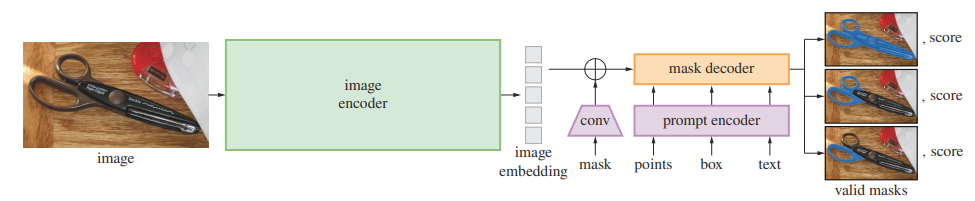
\includegraphics[width=\textwidth, height=0.45\textheight, keepaspectratio]{SAM.png}
    }{
        \begin{tikzpicture}
            \draw[dashed] (0,0) rectangle (\textwidth, 3) node[pos=.5] {Placeholder: SAM.png (Full Width)};
        \end{tikzpicture}
    }
\end{frame}

% Slide 9
\begin{frame}{The Semantic-Geometric Gap}
    \begin{block}{The Limitation of Scale (SA-1B Dataset)}
        SAM is trained on 1 billion high-quality masks, enforcing extreme geometric robustness. However, these masks are purely structural; they contain \textbf{no class or category labels}.
    \end{block}

    \begin{alertblock}{The Semantic Deficit}
        \begin{itemize}
            \item SAM learns \textit{"what constitutes an object"} but never learns \textit{"what the object is"}.
            \item It cannot natively process a support image-mask pair to locate a semantically identical object in a query image.
            \item External conditioning mechanisms must be engineered to translate semantic intent into SAM's native geometric prompt language.
        \end{itemize}
    \end{alertblock}
\end{frame}

% ==========================================
% SECTION 4: ENHANCED METHODOLOGIES
% ==========================================
\section{Methodological Taxonomies}

% Slide 10
\begin{frame}{Taxonomy of SAM-based Adaptation Strategies}
    \begin{table}[htbp]
    \centering
    \caption{Classification of Representative Few-Shot SAM Adaptation Methods}
    \renewcommand{\arraystretch}{1.05}
    \small
    \begin{tabular}{l p{0.55\linewidth}}
    \toprule
    \textbf{Paper} & \textbf{Adaptation Strategy} \\
    \midrule
    VRP-SAM (CVPR 2024) \cite{sun2024vrp} & Prompt-based adaptation (Automation) \\
    ProSAM (ICCV 2025) \cite{wang2025prosam} & Prompt-based (Probabilistic prompting) \\
    Matcher (IJCV 2025 / ICLR 2024) \cite{liu2023matcher} & Feature matching (Dense alignment) \\
    DC-SAM (TPAMI 2025) \cite{qi2025dcsam} & Consistency-based (Cyclic validation) \\
    Bridge the Points (NeurIPS 2024) \cite{zhang2024bridge} & Graph-based reasoning (Relational) \\
    FCP-SAM (AAAI 2025) \cite{park2025fcpsam} & Prototype-based modeling (Averaging) \\
    PerSAM (ICLR 2024) \cite{zhang2024persam} & Personalized adaptation (One-shot PEFT) \\
    DAPSAM (MICCAI 2024) \cite{wei2024prompting} \footnote{\tiny DAPSAM focuses on single-source domain generalization (SSDG) rather than typical FSS; it is included here as it generates task-specific prompts and adapts the SAM foundation model to the medical domain.} & Domain-adaptive prompting (Medical SSDG) \\
    \bottomrule
    \end{tabular}
    \end{table}
\end{frame}

% Slide 11: Architectural Overviews
\begin{frame}{Architectural Overviews: Key SAM Adaptations}
    \footnotesize
    \begin{columns}[T]
        \begin{column}{0.48\textwidth}
            \begin{itemize}
                \item \textbf{VRP-SAM:} Aux-encoder prompt automation. Efficient; sensitive to deformation.
                \item \textbf{ProSAM:} Multivariate prompt modeling. Boundary-robust; high latency.
                \item \textbf{Matcher:} Zero-shot DINOv2 cycle-consistency. Strong instance-level matching; susceptible to distractors.
                \item \textbf{DC-SAM:} Cyclic deviation checks. Mitigates semantic drift; high memory footprint.
            \end{itemize}
        \end{column}
        
        \begin{column}{0.48\textwidth}
            \begin{itemize}
                \item \textbf{Bridge-the-Points:} Directed graph clustering. Solves occlusion; $\mathcal{O}(|\mathcal{V}|^2)$ complexity in worst case.
                \item \textbf{FCP-SAM:} Dense prototype vectors. Strong multi-shot scaling; relies on aux-backbones.
                \item \textbf{PerSAM:} Target attention \& PEFT. Extremely lightweight; vulnerable to pose/lighting shifts.
                \item \textbf{DAPSAM:} Clinical domain prototypes. Handles fuzzy boundaries; increased latency.
            \end{itemize}
        \end{column}
    \end{columns}
\end{frame}
% ==========================================
% SECTION 5: DATASETS & EVALUATION METRICS
% ==========================================
\section{Datasets \& Evaluation}

% Slide 13
\begin{frame}{Evaluation Datasets \& Metrics Overview}
    \begin{block}{Dataset Categories}
        \begin{itemize}
            \item \textbf{Standard Baselines:} PASCAL-$5^i$, MS COCO-$20^i$ (Dense clutter).
            \item \textbf{Large Vocabulary:} FSS-1000, LVIS-$92^i$ (Long-tail distributions).
            \item \textbf{Part-Level Reasoning:} PASCAL-Part, PACO-Part (Intra-object boundaries).
            \item \textbf{Personalized \& Video:} PerSeg, DAVIS 2017 (Temporal tracking).
            \item \textbf{Medical SSDG:} Prostate MRI, RIGA+ Fundus (Low contrast, domain shift).
        \end{itemize}
    \end{block}
    
    \begin{block}{Evaluation Metrics Concept}
        \begin{itemize}
            \item \textbf{mIoU:} Measures overall spatial overlap between predicted and ground-truth masks.
            \item \textbf{Dice Score (DSC):} Heavily penalizes false positives/negatives; standard for medical.
            \item \textbf{Region Similarity ($\mathcal{J}$):} Evaluates spatial tracking overlap frame-by-frame in video.
            \item \textbf{Boundary Accuracy ($\mathcal{F}$):} Evaluates the strict contour precision of the object.
        \end{itemize}
    \end{block}
\end{frame}



% Slide 14
% Slide 25
\begin{frame}{Literature Results: Standard \& Large-Vocabulary Datasets}
    \vspace{-0.1cm}
    \begin{table}[htbp]
    \centering
    \caption{Overall Quantitative Results (mIoU \%)}
    \renewcommand{\arraystretch}{0.95} % Prevent vertical overflow
    \resizebox{\linewidth}{!}{
    \begin{tabular}{l l c c c c c c c c}
    \toprule
    \textbf{Method} & \textbf{Backbone} & \multicolumn{2}{c}{\textbf{PASCAL-5i}} & \multicolumn{2}{c}{\textbf{COCO-20i}} & \multicolumn{2}{c}{\textbf{FSS-1000}} & \multicolumn{2}{c}{\textbf{LVIS-92i}} \\
    \cmidrule(lr){3-4} \cmidrule(lr){5-6} \cmidrule(lr){7-8} \cmidrule(lr){9-10}
    & & \textbf{1-s} & \textbf{5-s} & \textbf{1-s} & \textbf{5-s} & \textbf{1-s} & \textbf{5-s} & \textbf{1-s} & \textbf{5-s} \\
    \midrule
    VRP-SAM \cite{sun2024vrp} & ResNet-50 & 71.9 & 72.9 & 53.9 & -- & -- & -- & -- & -- \\
    VRP-SAM \cite{sun2024vrp} & DINOv2 & -- & -- & 60.4 & -- & -- & -- & -- & -- \\
    ProSAM \cite{wang2025prosam} & ResNet-50 & 72.0 & -- & 54.6 & -- & -- & -- & -- & -- \\
    ProSAM \cite{wang2025prosam} & DINOv2 & -- & -- & 59.2 & -- & -- & -- & -- & -- \\
    Matcher \cite{liu2023matcher} & DINOv2 & -- & -- & 52.7 & 60.7 & 87.0 & \textbf{89.6} & 33.0 & 40.0 \\
    DC-SAM \cite{qi2025dcsam} & ResNet-50 & 73.0 & -- & 55.5 & -- & -- & -- & -- & -- \\
    DC-SAM \cite{qi2025dcsam} & DINOv2 & -- & -- & \textbf{62.0} & -- & -- & -- & -- & -- \\
    DC-SAM (SAM2) \cite{qi2025dcsam},\cite{ravi2024sam2} & ResNet-50 & \textbf{74.0} & -- & 56.4 & -- & -- & -- & -- & -- \\
    Bridge-the-Points \cite{zhang2024bridge} & DINOv2 & 72.1 & \textbf{82.6} & 58.7 & \textbf{66.8} & \textbf{88.0} & 88.9 & \textbf{35.2} & \textbf{44.2} \\
    FCP-SAM \cite{park2025fcpsam} & ResNet-50 & 73.2 & 74.0 & 52.5 & 58.0 & -- & -- & -- & -- \\
    \bottomrule
    \end{tabular}}
    \end{table}
\end{frame}

% Slide 15
\begin{frame}{Literature Results: Part-Level \& Backbone Impact}
    \begin{columns}[T]
        \begin{column}{0.48\textwidth}
            \begin{table}
                \caption{One-Shot Part Segmentation \cite{liu2023matcher, zhang2024bridge}}
                \resizebox{\linewidth}{!}{
                \begin{tabular}{l c c}
                \toprule
                \textbf{Method} & \textbf{PASCAL-Part} & \textbf{PACO-Part} \\
                \midrule
                Matcher & 42.9 & 34.7 \\
                Bridge-the-Points & \textbf{44.5} & \textbf{36.3} \\
                \bottomrule
                \end{tabular}}
            \end{table}
            \begin{alertblock}{Commentary}
                \footnotesize Part-level segmentation is significantly harder than whole-object extraction. Graph-based reasoning models structural relationships effectively.
            \end{alertblock}
        \end{column}
        
        \begin{column}{0.48\textwidth}
            \begin{table}
                \caption{Impact of Backbone on COCO (1-Shot)}
                \resizebox{\linewidth}{!}{
                \begin{tabular}{l c c c}
                \toprule
                \textbf{Method} & \textbf{ResNet-50} & \textbf{DINOv2} & \textbf{Gain} \\
                \midrule
                VRP-SAM & 53.9 & 60.4 & \textbf{+6.5} \\
                ProSAM & 54.6 & 59.2 & \textbf{+4.6} \\
                DC-SAM & 55.5 & 62.0 & \textbf{+6.5} \\
                \bottomrule
                \end{tabular}}
            \end{table}
            \begin{alertblock}{Commentary}
                \footnotesize The foundation-model encoder mathematically dictates the ultimate performance ceiling, with DINOv2 yielding massive, consistent gains.
            \end{alertblock}
        \end{column}
    \end{columns}
\end{frame}

% Slide 16
\begin{frame}{Literature Results: PerSAM \& DAPSAM Original Papers}
    \begin{columns}[T]
        \begin{column}{0.5\textwidth}
            \begin{table}
                \caption{Personalized \& Video Segmentation \cite{zhang2024persam}}
                \resizebox{\linewidth}{!}{
                \begin{tabular}{l l c c}
                \toprule
                \textbf{Method} & \textbf{Adaptation Type} & \textbf{PerSeg} & \textbf{DAVIS 2017} \\
                \midrule
                PerSAM & Training-Free & 89.3 & 66.9 \\
                PerSAM-F & PEFT (2 params) & \textbf{95.3} & \textbf{76.1} \\
                \bottomrule
                \end{tabular}}
            \end{table}
            \begin{alertblock}{Commentary}
                \footnotesize Fine-tuning merely 2 scale-aware parameters (PerSAM-F) dramatically recovers instance fidelity across static images and video tracking.
            \end{alertblock}
        \end{column}
        
        \begin{column}{0.5\textwidth}
            \begin{table}
                \caption{Domain Generalization on Medical Datasets \cite{wei2024prompting}}
                \resizebox{\linewidth}{!}{
                \begin{tabular}{l c c c c}
                \toprule
                \textbf{Method} & \textbf{Adaptation} & \textbf{Prostate} & \textbf{RIGA+(DOD)} & \textbf{RIGA+(DOC)} \\
                \midrule
                DAPSAM & Prototypes & \textbf{81.31} & \textbf{96.30} & \textbf{88.15} \\
                \bottomrule
                \end{tabular}}
            \end{table}
            \begin{alertblock}{Commentary}
                \footnotesize DAPSAM establishes a robust framework for clinical prompting, successfully navigating the severe domain shifts and low-contrast boundaries inherent in medical imaging.
            \end{alertblock}
        \end{column}
    \end{columns}
\end{frame}


% Slide 30
\begin{frame}{Complexity Trade-Offs}
    \footnotesize
    \begin{itemize}
        \item \textbf{Real-Time Efficiency:} Lightweight, single-pass methods (VRP-SAM) are fast but prone to fragmentation in complex scenes.
        \item \textbf{Intermediate Complexity:} Cross-image feature alignment (Matcher) introduces additional cost due to dense support-query interactions.
        \item \textbf{Probabilistic Prompting:} Modeling prompt uncertainty (ProSAM) improves robustness in ambiguous regions, at the cost of iterative sampling and increased inference time.
        \item \textbf{High Robustness, Higher Cost:} Multi-stage reasoning (DC-SAM, FCP-SAM) improves robustness at the expense of increased memory and latency.
        \item \textbf{Graph Bottleneck:} Structural graph-based methods (Bridge-the-Points) scale poorly with worst-case $\mathcal{O}(|\mathcal{V}|^2)$ complexity.
        \item \textbf{Personalized Adaptation Efficiency:} PerSAM is highly efficient but degrades under strong appearance shifts without refinement.
        \item \textbf{Domain Adaptation Overhead:} DAPSAM introduces additional modules to bridge distribution gaps, improving medical robustness but increasing computational cost compared to standard pipelines.
    \end{itemize}
\end{frame}


% ==========================================
% SECTION 8: DISCUSSION
% ==========================================
\section{Discussion and Research Gaps}

% Slide 1: Consolidated Discussion
\begin{frame}{Discussion and Key Insights}
    \begin{block}{Semantic Alignment \& Prompting}
        \footnotesize
        \begin{itemize}
            \item SAM's geometric prompts require explicit semantic correspondence to manage dense distractors (COCO, LVIS) and fine boundaries.
            \item Incorporating negative references resolves target-distractor ambiguities and mitigates overfitting to dominant multi-shot patterns.
        \end{itemize}
    \end{block}

    \begin{block}{Representations \& Computational Trade-Offs}
        \footnotesize
        \begin{itemize}
            \item Self-supervised transformers (e.g., DINOv2) establish a strictly higher performance ceiling compared to convolutional baselines.
            \item Multi-stage reasoning boosts accuracy in cluttered scenes but degrades latency and memory, necessitating dynamic, adaptive frameworks.
        \end{itemize}
    \end{block}
\end{frame}

% Slide 2: Consolidated Research Gaps
\begin{frame}{Research Gaps}
    \begin{alertblock}{Scalability \& Intrinsic Alignment Limitations}
        \footnotesize
        \begin{itemize}
            \item Iterative refinement and multi-stage graph constructions increase inference overhead, hindering deployment in resource-constrained settings.
            \item Current architectures heavily depend on complex auxiliary alignment modules; establishing intrinsic semantic correspondence directly within foundation encoders remains an open challenge.
        \end{itemize}
    \end{alertblock}
    
      \begin{alertblock}{The Multi-Shot Degradation Problem}
        \footnotesize
        \begin{itemize}
            \item Increasing support examples ($K>1$) sometimes underperforms one-shot baselines, as naive feature aggregation dilutes discriminative cues across pose or scale variations.
            \item Frameworks lack principled weighting mechanisms for contradictory support evidence, introducing severe processing bottlenecks.
        \end{itemize}
    \end{alertblock}
\end{frame}







% ==========================================
% SECTION 7: COMPLETED WORK IN PHD
% ==========================================
\section{Completed Work in PhD}

% Slide 17
\begin{frame}{1. VRP-SAM: Baseline Reproduction (PASCAL \& COCO)}
    \begin{columns}[T]
        \begin{column}{0.48\textwidth}
            \begin{table}
                \caption{PASCAL-$5^i$ Reproduction (ResNet-50)}
                \resizebox{\linewidth}{!}{
                \begin{tabular}{l c c c}
                \toprule
                \textbf{Split} & \textbf{Paper (\%)} & \textbf{Reprod. (\%)} & \textbf{$\Delta$} \\
                \midrule
                Fold 0 & 73.9 & 73.69 & $-0.21$ \\
                Fold 1 & 78.3 & 76.60 & $-1.70$ \\
                Fold 2 & 70.6 & 68.01 & $-2.59$ \\
                Fold 3 & 65.0 & 63.38 & $-1.62$ \\
                \midrule
                \textbf{Mean} & \textbf{72.0} & \textbf{70.42} & \textbf{$-1.53$} \\
                \bottomrule
                \end{tabular}}
            \end{table}
        \end{column}
        
        \begin{column}{0.48\textwidth}
            \begin{table}
                \caption{COCO-$20^i$ Reproduction (ResNet-50, Mask)}
                \resizebox{\linewidth}{!}{
                \begin{tabular}{l c c c}
                \toprule
                \textbf{Split} & \textbf{Paper (\%)} & \textbf{Reprod. (\%)} & \textbf{$\Delta$} \\
                \midrule
                Fold 0 & 48.1 & 43.57 & $-4.53$ \\
                Fold 1 & 55.8 & 54.05 & $-1.75$ \\
                Fold 2 & 60.0 & 53.44 & $-6.56$ \\
                \bottomrule
                \end{tabular}}
            \end{table}
        \end{column}
    \end{columns}

    \vspace{0.3cm}
    \begin{alertblock}{Commentary}
        \footnotesize The reproduction accurately tracks the paper's performance distribution across folds, validating the structural integrity of our local implementation pipeline before enhancements.
    \end{alertblock}
\end{frame}


\begin{frame}{1. VRP-SAM: Model Soup Architecture (Enhancement) \cite{wasfy2023enhancing} }
    \begin{figure}[h]
        \centering
        \IfFileExists{model_soup.png}{
            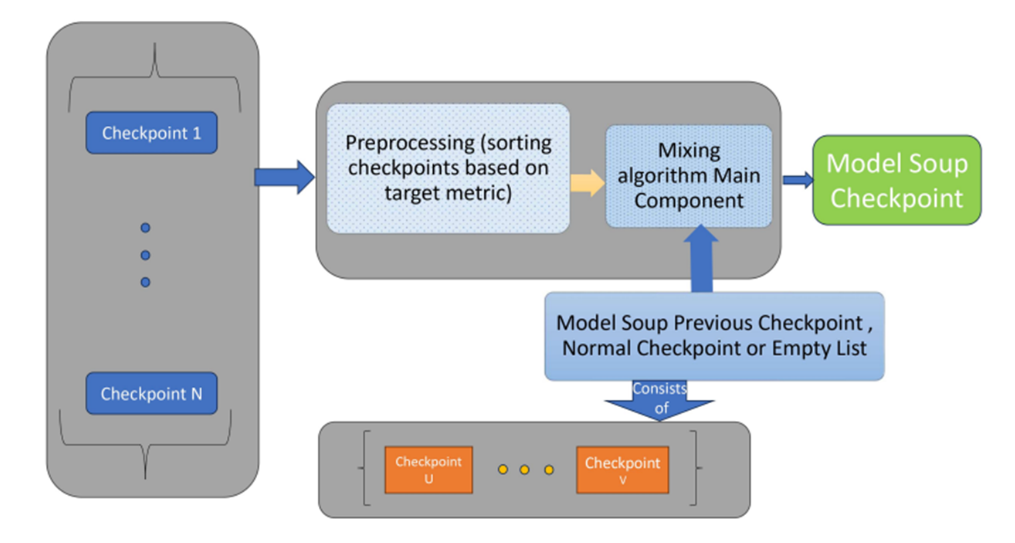
\includegraphics[width=\textwidth, height=0.85\textheight, keepaspectratio]{model_soup.png}
        }{
            \begin{tikzpicture}
                \draw[dashed] (0,0) rectangle (\textwidth, 4) node[pos=.5] {Placeholder: model_soup.png (Full Width)};
            \end{tikzpicture}
        }
    \end{figure}
\end{frame}

% Slide 18

\begin{frame}{1. VRP-SAM: Iterative Model Soup Enhancements}
    \begin{block}{Methodology}
        We applied an \textbf{Iterative Uniform Greedy Soup and Standard Greedy Soup} \cite{wasfy2023enhancing},\cite{wortsman2022modelsoups} to dynamically average weights across fine-tuning checkpoints, seeking to smooth the loss landscape without adding inference latency.
    \end{block}

    \vspace{-0.2cm}
    \begin{table}[htbp]
    \centering
    \caption{VRP-SAM Model Soup Enhancements on COCO Dataset (ResNet-50, mIoU \%)}
    \label{tab:vrp_sam_soup}
    \resizebox{0.95\linewidth}{!}{
    \begin{tabular}{l l c c c c}
    \toprule
    \textbf{Label Type} & \textbf{Split} & \textbf{Baseline (Reprod.)} & \textbf{Standard Soup} & \textbf{Iterative Greedy Soup} & \textbf{$\Delta$ (Best - Baseline)} \\
    \midrule
    Point    & Fold-0 & 29.11 & 29.20 & 29.20 & +0.09 \\
    Scribble & Fold-0 & 44.22 & 44.37 & 44.37 & +0.15 \\
    Box      & Fold-0 & 39.71 & 39.84 & 39.84 & +0.13 \\
    Mask     & Fold-0 & 43.57 & 44.00 & 44.00 & +0.43 \\
    Mask     & Fold-1 & 54.05 & 54.21 & 54.34 & +0.29 \\
    Mask     & Fold-2 & 53.44 & 53.52 & 53.52 & +0.08 \\
    \bottomrule
    \end{tabular}}
    \end{table}
    
    \vspace{-0.2cm}
    \begin{alertblock}{Commentary}
        \footnotesize Capturing diverse feature representations from different epochs prevented overfitting to the sparse 1-shot support set, yielding a robust, "free" absolute gain up to +0.43\% without modifying the frozen SAM backbone.
    \end{alertblock}
\end{frame}

% Slide 19
\begin{frame}{2. Bridge the Points (GF-SAM): Baseline Reproduction (PASCAL \& COCO)}
    \begin{columns}[T]
        \begin{column}{0.5\textwidth}
            \begin{table}
                \caption{PASCAL-$5^i$ (mIoU \%)}
                \resizebox{\linewidth}{!}{
                \begin{tabular}{l c c c c}
                \toprule
                \multirow{2}{*}{\textbf{Split}} & \multicolumn{2}{c}{\textbf{1-Shot}} & \multicolumn{2}{c}{\textbf{5-Shot}} \\
                \cmidrule(lr){2-3} \cmidrule(lr){4-5}
                & \textbf{Pap.} & \textbf{Rep.} & \textbf{Pap.} & \textbf{Rep.} \\
                \midrule
                Fold 0 & -- & 70.84 & -- & 81.49 \\
                Fold 1 & -- & 75.65 & -- & 86.39 \\
                Fold 2 & -- & 69.14 & -- & 79.53 \\
                Fold 3 & -- & 72.75 & -- & 82.64 \\
                \midrule
                \textbf{Avg} & \textbf{72.1} & \textbf{72.10} & \textbf{82.6} & \textbf{82.51} \\
                \bottomrule
                \end{tabular}}
            \end{table}
        \end{column}
        
        \begin{column}{0.5\textwidth}
            \begin{table}
                \caption{COCO-$20^i$ (mIoU \%)}
                \resizebox{\linewidth}{!}{
                \begin{tabular}{l c c c c}
                \toprule
                \multirow{2}{*}{\textbf{Split}} & \multicolumn{2}{c}{\textbf{1-Shot}} & \multicolumn{2}{c}{\textbf{5-Shot}} \\
                \cmidrule(lr){2-3} \cmidrule(lr){4-5}
                & \textbf{Pap.} & \textbf{Rep.} & \textbf{Pap.} & \textbf{Rep.} \\
                \midrule
                Fold 0 & -- & 56.71 & -- & 67.11 \\
                Fold 1 & -- & -- & -- & 70.33 \\
                Fold 2 & -- & 59.70 & -- & 65.81 \\
                Fold 3 & -- & 57.20 & -- & 65.40 \\
                \midrule
                \textbf{Avg} & \textbf{58.7} & \textbf{57.87} & \textbf{66.8} & \textbf{67.16} \\
                \bottomrule
                \end{tabular}}
            \end{table}
        \end{column}
    \end{columns}

   
\end{frame}

% Slide 20
\begin{frame}{3. PerSAM: Aggregated PerSeg \& DAVIS Reproduction}
    \begin{table}[htbp]
    \centering
    \caption{Aggregated Metrics: PerSAM vs PerSAM-F on PerSeg}
    \resizebox{0.8\linewidth}{!}{
    \begin{tabular}{l c c c c c c}
    \toprule
    \textbf{Metric} & \textbf{Paper PerSAM} & \textbf{Reprod. PerSAM} & \textbf{$\Delta$} & \textbf{Paper PerSAM-F} & \textbf{Reprod. PerSAM-F} & \textbf{$\Delta$} \\
    \midrule
    mIoU & 89.3\% & 89.32\% & +0.02\% & 95.3\% & 95.18\% & $-0.12\%$ \\
    \bottomrule
    \end{tabular}}
    \end{table}

    \begin{table}[htbp]
    \centering
    \caption{DAVIS-2017: Global Validation Results (Reproduced vs Paper)}
    \resizebox{0.85\linewidth}{!}{
    \begin{tabular}{l c c c c c c}
    \toprule
    \textbf{Metric} & \textbf{PerSAM (Rep.)} & \textbf{PerSAM-F (Rep.)} & \textbf{Rep. Gain} & \textbf{PerSAM (Pap.)} & \textbf{PerSAM-F (Pap.)} & \textbf{Pap. Gain} \\
    \midrule
    Mean ($\mathcal{J}\&\mathcal{F}$) & 58.98\% & 70.00\% & +11.02\% & 66.9\% & 76.1\% & +9.2\% \\
    Mean $\mathcal{J}$ & 55.11\% & 67.02\% & +11.91\% & 63.4\% & 73.2\% & +9.8\% \\
    Mean $\mathcal{F}$ & 62.85\% & 72.98\% & +10.13\% & 70.4\% & 78.9\% & +8.5\% \\
    \bottomrule
    \end{tabular}}
    \end{table}

    \begin{alertblock}{Commentary}
        \footnotesize PerSeg reproduction was nearly identical to published data. While raw DAVIS absolute scores were lower due to hardware mapping variances, the \textbf{delta gain} achieved via fine-tuning (+11.02\%) significantly exceeded the paper's reported improvements, thoroughly validating the PEFT paradigm.
    \end{alertblock}
\end{frame}

% Slide 21
\begin{frame}{3. PerSAM: Enhancements on PerSeg}
    \begin{block}{Dual-Stream DINOv2 Fusion}
        Standard PerSAM collapses on low-texture or similar-colored objects. We fused high-capacity global semantics (\texttt{dinov2.lvd142m}) with SAM's geometric similarities, added Gaussian mask smoothing, and optimized bounding-box padding margins.
    \end{block}

    \begin{table}[htbp]
    \centering
    \caption{Enhanced PerSAM vs Reproduced Baseline on PerSeg}
    \resizebox{0.6\linewidth}{!}{
    \begin{tabular}{l c c c}
    \toprule
    \textbf{Metric} & \textbf{Reproduced (mIoU \%)} & \textbf{Enhanced (mIoU \%)} & \textbf{$\Delta$} \\
    \midrule
    Overall Mean & 89.32\% & 91.12\% & \textbf{+1.80\%} \\
    \bottomrule
    \end{tabular}}
    \end{table}

    \begin{alertblock}{Commentary}
        \footnotesize This dual-stream enhancement successfully overrides SAM's geometric bias, recovering massive performance on visually ambiguous failure cases without modifying the target object itself.
    \end{alertblock}
\end{frame}

% Slide 22
\begin{frame}{3. PerSAM-F: Enhancements on PerSeg}
    \begin{block}{Fine-Tuning Structural Stability}
        Enhancements to the fine-tuning pipeline prioritized structural stability via fixed-resolution optimization normalization (\texttt{train\_resolution 256}) and cascading context margins (\texttt{box\_padding 0.03}).
    \end{block}

    \begin{table}[htbp]
    \centering
    \caption{Enhanced PerSAM-F vs Reproduced Baseline on PerSeg}
    \resizebox{0.6\linewidth}{!}{
    \begin{tabular}{l c c c}
    \toprule
    \textbf{Metric} & \textbf{Reproduced (mIoU \%)} & \textbf{Enhanced (mIoU \%)} & \textbf{$\Delta$} \\
    \midrule
    Overall Mean & 95.18\% & 95.60\% & \textbf{+0.42\%} \\
    \bottomrule
    \end{tabular}}
    \end{table}
\end{frame}

% Slide 23
\begin{frame}{3. PerSAM: Temporal Enhancements on DAVIS}
    \begin{block}{Temporal Memory Bank \& Confidence-Gating}
        To address video tracking drift, we cached recent target feature vectors (\texttt{memory\_size=3}) and conditionally gated updates exclusively on highly confident frames (score $> 0.7$).
    \end{block}

    \begin{table}[htbp]
    \centering
    \caption{Enhanced PerSAM-Video Performance on DAVIS 2017}
    \resizebox{0.6\linewidth}{!}{
    \begin{tabular}{l c c c}
    \toprule
    \textbf{Metric} & \textbf{Reproduced (\%)} & \textbf{Enhanced (\%)} & \textbf{$\Delta$} \\
    \midrule
    Mean ($\mathcal{J}\&\mathcal{F}$) & 58.98\% & 61.18\% & +2.20\% \\
    Mean $\mathcal{J}$ & 55.11\% & 57.43\% & +2.32\% \\
    Mean $\mathcal{F}$ & 62.85\% & 64.93\% & +2.08\% \\
    \bottomrule
    \end{tabular}}
    \end{table}

    \begin{alertblock}{Commentary}
        \footnotesize This memory-gated temporal framework effectively suppresses the accumulation of erroneous feature drift caused by motion blur, dramatically recovering performance on highly dynamic sequences.
    \end{alertblock}
\end{frame}


\begin{frame}{3. PerSAM: SAM3 Text-Prompted Pipeline }
    \begin{figure}[h]
        \centering
        \IfFileExists{SAM3.png}{
            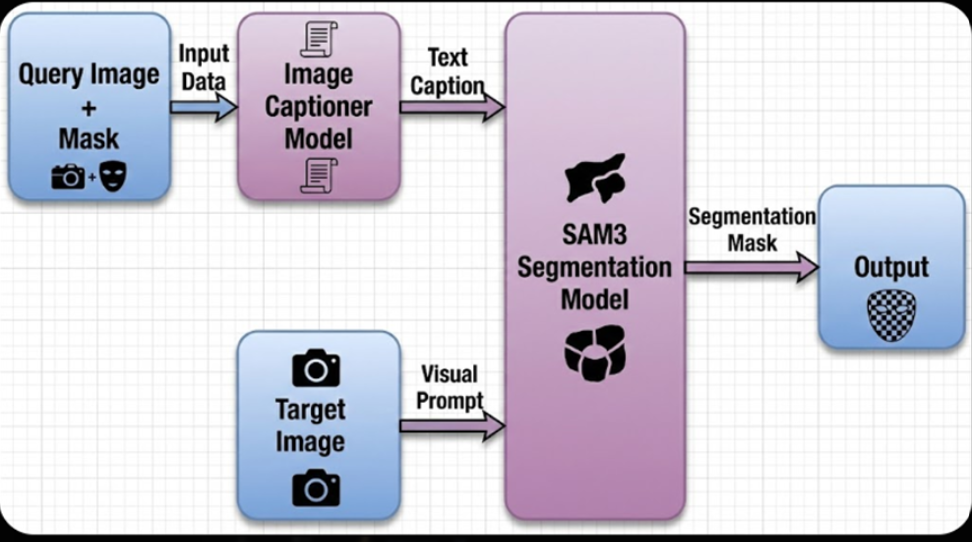
\includegraphics[width=\textwidth, height=0.85\textheight, keepaspectratio]{SAM3.png}
        }{
            \begin{tikzpicture}
                \draw[dashed] (0,0) rectangle (\textwidth, 4) node[pos=.5] {Placeholder: SAM3.png (Full Width)};
            \end{tikzpicture}
        }
    \end{figure}
\end{frame}

% Slide 24
\begin{frame}{3. PerSAM: SAM3 Text-Prompted Pipeline Evaluation}
    \begin{block}{Experimental Setup}
        To assess if PerSeg objects genuinely demand visual personalization, a novel SAM3\cite{carion2025sam3} pipeline was tested using \textbf{only manual text descriptions} (e.g., \textit{"silver beverage can"}).
    \end{block}

    \begin{table}[htbp]
    \centering
    \caption{Aggregated Comparison: SAM3 vs PerSAM Frameworks}
    \resizebox{0.8\linewidth}{!}{
    \begin{tabular}{l c | c c | c c}
    \toprule
    \textbf{Metric} & \textbf{SAM3 (Text)} & \textbf{Rep. PerSAM} & \textbf{$\Delta$ (vs PerSAM)} & \textbf{Rep. PerSAM-F} & \textbf{$\Delta$ (vs PerSAM-F)} \\
    \midrule
    mIoU & 95.15\% & 89.32\% & +5.83\% & 95.18\% & $-0.03\%$ \\
    \bottomrule
    \end{tabular}}
    \end{table}
    
    \begin{alertblock}{Commentary}
        \footnotesize Remarkably, the purely text-guided SAM3 pipeline effectively tied the heavily mathematically optimized PerSAM-F pipeline. This indicates that objects within the PerSeg dataset can largely be resolved via explicit text descriptions rather than requiring deep, latent-space visual personalization, revealing a structural limitation of the benchmark itself.
    \end{alertblock}
\end{frame}

% Slide 25
\begin{frame}{4. DAPSAM: Medical Domain Enhancements (Prostate)}
    \begin{block}{Structural Refinements}
        \begin{itemize}
            \item \textbf{Residual Scaling:} Dynamically balances pre-trained priors with learned medical features.
            \item \textbf{Dropout (0.1) \& MLP Ratio (0.25):} Regularization to mitigate clinical dataset overfitting.
        \end{itemize}
    \end{block}

    \begin{table}[htbp]
    \centering
    \caption{Prostate MRI: Original, Reproduced, and Enhanced DAPSAM}
    \resizebox{0.9\linewidth}{!}{
    \begin{tabular}{l c c c c c c c c c}
    \toprule
    \textbf{Domain} & \textbf{Orig. Dice} & \textbf{Repr. Dice} & \textbf{$\Delta$(R-O)} & \textbf{Repr. ASD} & \textbf{Enh. Dice} & \textbf{$\Delta$(E-R)} & \textbf{$\Delta$(E-O)} & \textbf{Enh. ASD} & \textbf{$\Delta$ASD (E-R)} \\
    \midrule
    A & 86.34 & 85.48 & $-0.86$ & 2.60 & 86.71 & +1.23 & +0.37 & 2.08 & $-0.52$ \\
    B & 81.05 & 80.62 & $-0.43$ & 7.53 & 80.40 & $-0.22$ & $-0.65$ & 7.07 & $-0.46$ \\
    C & 70.81 & 64.99 & $-5.82$ & 6.12 & 68.58 & +3.59 & $-2.23$ & 6.34 & +0.22 \\
    D & 85.28 & 84.53 & $-0.75$ & 2.46 & 84.49 & $-0.04$ & $-0.79$ & 2.42 & $-0.04$ \\
    E & 82.91 & 83.13 & +0.22 & 4.30 & 83.53 & +0.40 & +0.62 & 3.80 & $-0.50$ \\
    F & 81.48 & 79.57 & $-1.91$ & 6.51 & 81.14 & +1.57 & $-0.34$ & 5.67 & $-0.84$ \\
    \midrule
    \textbf{Avg} & \textbf{81.31} & \textbf{79.72} & \textbf{$-1.59$} & \textbf{4.59} & \textbf{80.81} & \textbf{+1.09} & \textbf{$-0.50$} & \textbf{4.23} & \textbf{$-0.36$} \\
    \bottomrule
    \end{tabular}}
    \end{table}
    
   
\end{frame}

% Slide 26
\begin{frame}{4. DAPSAM: Medical Domain Enhancements (RIGA+)}
    \begin{table}[htbp]
    \centering
    \caption{RIGA+ BinRushed: Reproduced vs Enhanced (Dice Score \%)}
    \resizebox{0.75\linewidth}{!}{
    \begin{tabular}{l c c c c c c}
    \toprule
    \textbf{Target} & \textbf{Orig. Avg} & \textbf{Repr.} & \textbf{$\Delta$(Repr-Orig)} & \textbf{Enh.} & \textbf{$\Delta$(Enh-Repr)} & \textbf{$\Delta$(Enh-Orig)} \\
    \midrule
    \textbf{DOD Avg} & 96.26 & 96.11 & $-0.15$ & 96.08 & $-0.03$ & $-0.18$ \\
    \textbf{DOC Avg} & 87.87 & 85.78 & $-2.09$ & 86.70 & \textbf{+0.92} & $-1.17$ \\
    \bottomrule
    \end{tabular}}
    \end{table}

    \begin{table}[htbp]
    \centering
    \caption{RIGA+ Magrabia: Reproduced vs Enhanced (Dice Score \%)}
    \resizebox{0.75\linewidth}{!}{
    \begin{tabular}{l c c c c c c}
    \toprule
    \textbf{Target} & \textbf{Orig. Avg} & \textbf{Repr.} & \textbf{$\Delta$(Repr-Orig)} & \textbf{Enh.} & \textbf{$\Delta$(Enh-Repr)} & \textbf{$\Delta$(Enh-Orig)} \\
    \midrule
    \textbf{DOD Avg} & 96.30 & 95.56 & $-0.74$ & 95.54 & $-0.02$ & $-0.76$ \\
    \textbf{DOC Avg} & 88.15 & 88.05 & $-0.10$ & 88.32 & \textbf{+0.27} & +0.17 \\
    \bottomrule
    \end{tabular}}
    \end{table}

    \begin{alertblock}{Commentary}
\footnotesize
The Optic Cup (DOC) has weaker boundaries than the Optic Disc (DOD), increasing sensitivity to domain shift. The enhancements reduce this effect, yielding gains of +0.92\% (BinRushed) and +0.27\% (Magrabia), and improving feature stability in ambiguous regions.
\end{alertblock}
    
\end{frame}



% ==========================================
% SECTION 10: PROPOSED DIRECTIONS
% ==========================================
\section{Proposed PhD Research Directions}

% Slide 1: Consolidated Proposed Directions
\begin{frame}{Proposed Research Directions \& Contributions}
    \begin{columns}[T]
        \begin{column}{0.48\textwidth}
            \begin{block}{Methodology \& Adaptation}
                \footnotesize
                \begin{itemize}
                    \item \textbf{Robust Alignment:} Integrate uncertainty-aware prompt weighting and lightweight cross-image feature matching.
                    \item \textbf{Efficient Modules:} Design parameter-efficient adapters for a frozen SAM backbone to minimize overhead.
                    \item \textbf{Complexity Handling:} Enforce spatial consistency to suppress distractors in cluttered datasets (e.g., COCO-$20^i$).
                \end{itemize}
            \end{block}
        \end{column}
        
        \begin{column}{0.48\textwidth}
            \begin{block}{Deployment \& Key Contributions}
                \footnotesize
                \begin{itemize}
                    \item \textbf{Resource Optimization:} Minimize inference latency and memory footprint to ensure feasibility on constrained hardware.
                    \item \textbf{Expected Outcomes:}
                    \begin{itemize}
                        \footnotesize
                        \item A novel, lightweight conditioning framework for SAM-based FSS.
                        \item Systematic failure mode analysis in complex visual environments.
                        \item Reproducible benchmarks under standardized evaluation protocols.
                    \end{itemize}
                \end{itemize}
            \end{block}
        \end{column}
    \end{columns}
\end{frame}
% Slide 36
\begin{frame}{Research Plan and Phases}
    \begin{columns}[T]
        \begin{column}{0.48\textwidth}
            \begin{block}{Phase 1: Baseline Benchmarking}
                \scriptsize
                \begin{itemize}
                    \item Reproduce core baselines (VRP-SAM, ProSAM, DC-SAM, PerSAM, etc.).
                    \item Standardize protocols and unified metrics (mIoU, Dice, FPS).
                \end{itemize}
            \end{block}
            \begin{block}{Phase 2: Failure Mode Analysis}
                \scriptsize
                \begin{itemize}
                    \item Analyze boundary region failures and distractor confusion.
                    \item Identify computational bottlenecks.
                \end{itemize}
            \end{block}
            \begin{block}{Phase 3: Method Development}
                \scriptsize
                \begin{itemize}
                    \item Design a lightweight conditioning framework.
                    \item Introduce mechanisms for robustness (e.g., prompt refinement).
                \end{itemize}
            \end{block}
        \end{column}
        
        \begin{column}{0.48\textwidth}
            \begin{block}{Phase 4: Extended Evaluation}
                \scriptsize
                \begin{itemize}
                    \item Conduct ablation studies on individual components.
                    \item Test generalization on FSS-1000 and LVIS-$92^i$.
                \end{itemize}
            \end{block}
            \begin{block}{Phase 5: Efficiency Optimization}
                \scriptsize
                \begin{itemize}
                    \item Optimize inference pipeline for reduced latency/memory.
                    \item Explore deployment on constrained hardware.
                \end{itemize}
            \end{block}
            \begin{block}{Phase 6: Thesis Consolidation}
                \scriptsize
                \begin{itemize}
                    \item Integrate results into a unified framework.
                    \item Prepare publications targeting top-tier venues (CVPR, TPAMI).
                \end{itemize}
            \end{block}
        \end{column}
    \end{columns}
\end{frame}

% ==========================================
% SECTION 12: CONCLUSION
% ==========================================
\section{Conclusion}

% Slide 37
\begin{frame}{Conclusion}
    \begin{exampleblock}{Synthesis \& Final Objective}
        \footnotesize
        \begin{itemize}
            \item This proposal consolidates recent related work, the full body of work completed in the PhD so far (VRP-SAM, GF-SAM, PerSAM, DAPSAM), and the unified comparative methodology.
            \item The foundation for a highly robust, reference-guided segmentation system utilizing foundation models has been firmly established.
            \item The extensive reproductions demonstrate that the inherent architectural rigidity of models like SAM can be effectively circumvented via mathematically rigorous conditioning mechanisms and domain-adaptive prototypes.
            \item \textbf{Future Objective:} Extend these frameworks toward fully trustworthy, uncertainty-aware, and deployment-ready visual perception systems under real-world conditions and extreme domain shifts.
        \end{itemize}
    \end{exampleblock}
\end{frame}

% ==========================================
% REFERENCES
% ==========================================
\begin{frame}[allowframebreaks]{References}
    \bibliographystyle{IEEEtran}
    \begin{thebibliography}{10}
\bibitem{kirillov2023segment}
Kirillov, A., Mintun, E., Ravi, N., Mao, H., Rolland, C., Gustafson, L., ... \& Girshick, R. (2023). Segment anything. In \textit{Proceedings of the IEEE/CVF International Conference on Computer Vision} (pp. 4015-4026).

\bibitem{he2016deep}
He, K., Zhang, X., Ren, S., \& Sun, J. (2016). Deep residual learning for image recognition. In \textit{Proceedings of the IEEE conference on computer vision and pattern recognition} (pp. 770-778).

\bibitem{oquab2023dinov2}
Oquab, M., Darcet, T., Moutakanni, T., Vo, H., Szafraniec, M., Khalidov, V., ... \& Bojanowski, P. (2023). Dinov2: Learning robust visual features without supervision. \textit{arXiv preprint arXiv:2304.07193}.

\bibitem{dosovitskiy2020image}
Dosovitskiy, A., Beyer, L., Kolesnikov, A., Weissenborn, D., Zhai, X., Unterthiner, T., ... \& Houlsby, N. (2020). An image is worth 16x16 words: Transformers for image recognition at scale. \textit{International Conference on Learning Representations}.

\bibitem{shaban2017one}
Shaban, A., Bansal, S., Liu, Z., Essa, I., \& Boots, B. (2017). One-shot learning for semantic segmentation. In \textit{Proceedings of the British Machine Vision Conference (BMVC)}.

\bibitem{nguyen2019feature}
Nguyen, K., \& Todorovic, S. (2019). Feature weighting and boosting for few-shot segmentation. In \textit{Proceedings of the IEEE/CVF International Conference on Computer Vision} (pp. 622-631).

\bibitem{everingham2010pascal}
Everingham, M., Van Gool, L., Williams, C. K., Winn, J., \& Zisserman, A. (2010). The pascal visual object classes (voc) challenge. \textit{International journal of computer vision}, 88(2), 303-338.

\bibitem{lin2014microsoft}
Lin, T. Y., Maire, M., Belongie, S., Hays, J., Perona, P., Ramanan, D., ... \& Zitnick, C. L. (2014). Microsoft coco: Common objects in context. In \textit{European conference on computer vision} (pp. 740-755). Springer, Cham.

\bibitem{li2020fss}
Li, X., Wei, T., Chen, Y. P., Tai, Y.-W., \& Tang, C.-K. (2020). Fss-1000: A 1000-class dataset for few-shot segmentation. In \textit{Proceedings of the IEEE/CVF conference on computer vision and pattern recognition} (pp. 2869-2878).

\bibitem{gupta2019lvis}
Gupta, A., Dollar, P., \& Girshick, R. (2019). Lvis: A dataset for large vocabulary instance segmentation. In \textit{Proceedings of the IEEE/CVF conference on computer vision and pattern recognition} (pp. 5356-5364).

\bibitem{chen2014detect}
Chen, X., Mottaghi, R., Liu, X., Fidler, S., Urtasun, R., \& Yuille, A. (2014). Detect what you can: Detecting and representing objects using holistic models and body parts. In \textit{Proceedings of the IEEE conference on computer vision and pattern recognition} (pp. 1971-1978).

\bibitem{ramanathan2023paco}
Ramanathan, V., Kalia, A., Petrovic, V., Wen, Y., Zheng, B., Guo, B., ... \& Marquez, A. (2023). Paco: Parts and attributes of common objects. \textit{arXiv preprint arXiv:2301.01795}.

\bibitem{wang2019panet}
Wang, K., Liew, J. H., Zou, Y., Zhou, D., \& Feng, J. (2019). PANet: Few-shot image semantic segmentation with prototype alignment. In \textit{Proceedings of the IEEE/CVF International Conference on Computer Vision} (pp. 9197-9206).

\bibitem{tian2020pfenet}
Tian, Z., Zhao, H., Shu, M., Yang, Z., Li, R., \& Jia, J. (2020). Prior guided feature enrichment network for few-shot segmentation. \textit{IEEE Transactions on Pattern Analysis and Machine Intelligence}, 44(2), 1050-1065.

\bibitem{sun2024vrp}
Sun, Y., Chen, J., Zhang, S., Zhang, X., Chen, Q., Zhang, G., \& Li, Z. (2024).
VRP-SAM: SAM with visual reference prompt.
In \textit{Proceedings of the IEEE/CVF Conference on Computer Vision and Pattern Recognition (CVPR)} (pp. 23565--23574).

\bibitem{wang2025prosam}
Wang, X., Sebastian, C., He, W., \& Ren, L. (2025).
ProSAM: Enhancing the robustness of SAM-based visual reference segmentation with probabilistic prompts.
In \textit{Proceedings of the IEEE/CVF International Conference on Computer Vision (ICCV)} (pp. 20487--20496).

\bibitem{liu2023matcher}
Liu, Y., Zhu, M., Li, H., Chen, H., Wang, X., \& Shen, C. (2023).
Matcher: Segment anything with one shot using all-purpose feature matching.
\textit{arXiv preprint arXiv:2305.13310}.

\bibitem{qi2025dcsam}
Qi, M., Zhu, P., Li, X., Bi, X., Qi, L., Ma, H., \& Yang, M. H. (2025).
DC-SAM: In-context segment anything in images and videos via dual consistency.
\textit{IEEE Transactions on Pattern Analysis and Machine Intelligence}.

\bibitem{zhang2024bridge}
Zhang, A., Gao, G., Jiao, J., Liu, C., \& Wei, Y. (2024).
Bridge the points: Graph-based few-shot segment anything semantically.
In \textit{Advances in Neural Information Processing Systems (NeurIPS)}, 37, 33232--33261.

\bibitem{park2025fcpsam}
Park, S., Lee, S., Seong, H. S., Yoo, J., \& Heo, J. P. (2025).
Foreground-covering prototype generation and matching for SAM-aided few-shot segmentation.
In \textit{Proceedings of the AAAI Conference on Artificial Intelligence}, 39(6), 6425--6433.

\bibitem{zhang2024persam}
Zhang, R., Jiang, Z., Guo, Z., Yan, S., Pan, J., Dong, H., ... \& Gao, P. (2024). 
Personalize segment anything model with one shot.
In \textit{International Conference on Learning Representations (ICLR)}.

\bibitem{wei2024prompting}
Wei, Z., Dong, W., Zhou, P., Gu, Y., Zhao, Z., \& Xu, Y. (2024). 
Prompting segment anything model with domain-adaptive prototype for generalizable medical image segmentation. 
In \textit{International conference on medical image computing and computer-assisted intervention} (pp. 533--543). Springer.

\bibitem{pont2017the}
Pont-Tuset, J., Perazzi, F., Marques, S., Garcia, J., \& Van Gool, L. (2017). 
The 2017 davis challenge on video object segmentation. 
\textit{arXiv preprint arXiv:1704.00675}.

\bibitem{ravi2024sam2}
Ravi, N., Gabeur, V., Hu, Y. T., Hu, R., Ryali, C., Ma, T., \& Feichtenhofer, C. (2024).
SAM 2: Segment anything in images and videos.
\textit{arXiv preprint arXiv:2408.00714}.

\bibitem{carion2025sam3}
Carion, N., Gustafson, L., Hu, Y. T., Debnath, S., Hu, R., Suris, D., \& Feichtenhofer, C. (2025).
SAM 3: Segment anything with concepts.
\textit{arXiv preprint arXiv:2511.16719}.

\bibitem{wortsman2022modelsoups}
Wortsman, M., Ilharco, G., Gadre, S. Y., Roelofs, R., Gontijo-Lopes, R., Morcos, A. S., \& Schmidt, L. (2022).
Model soups: Averaging weights of multiple fine-tuned models improves accuracy without increasing inference time.
In \textit{Proceedings of the 39th International Conference on Machine Learning (ICML)} (pp. 23965--23998). PMLR.

\bibitem{wasfy2023enhancing}
Wasfy, O., Basiony, S., \& Torki, M. (2023).
Enhancing LiDAR Semantic Segmentation Using Model Soups.
In \textit{2023 20th ACS/IEEE International Conference on Computer Systems and Applications (AICCSA)} (pp. 1--7). IEEE.


 \end{thebibliography}
\end{frame}

% Slide 48 (Thank You Slide)
\begin{frame}
    \frametitle{Thank You}
    \vfill
    \centering
    \IfFileExists{thankyou.png}{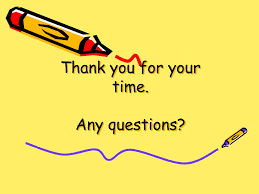
\includegraphics[width=1\linewidth,height=0.79\textheight,keepaspectratio]{thankyou.png}}{[Placeholder: thankyou.png]}
    
    \begin{flushright}
        \tiny\textbf{Email: omar.wasfy@alexu.edu.eg}
    \end{flushright}
    \vfill
\end{frame}

\end{document}